\documentclass[]{article}
\usepackage{lmodern}
\usepackage{amssymb,amsmath}
\usepackage{ifxetex,ifluatex}
\usepackage{fixltx2e} % provides \textsubscript
\ifnum 0\ifxetex 1\fi\ifluatex 1\fi=0 % if pdftex
  \usepackage[T1]{fontenc}
  \usepackage[utf8]{inputenc}
\else % if luatex or xelatex
  \ifxetex
    \usepackage{mathspec}
  \else
    \usepackage{fontspec}
  \fi
  \defaultfontfeatures{Ligatures=TeX,Scale=MatchLowercase}
\fi
% use upquote if available, for straight quotes in verbatim environments
\IfFileExists{upquote.sty}{\usepackage{upquote}}{}
% use microtype if available
\IfFileExists{microtype.sty}{%
\usepackage{microtype}
\UseMicrotypeSet[protrusion]{basicmath} % disable protrusion for tt fonts
}{}
\usepackage[margin=1in]{geometry}
\usepackage{hyperref}
\hypersetup{unicode=true,
            pdftitle={Texas Housing Prices: latex\_document},
            pdfauthor={Alison Hill},
            pdfborder={0 0 0},
            breaklinks=true}
\urlstyle{same}  % don't use monospace font for urls
\usepackage{color}
\usepackage{fancyvrb}
\newcommand{\VerbBar}{|}
\newcommand{\VERB}{\Verb[commandchars=\\\{\}]}
\DefineVerbatimEnvironment{Highlighting}{Verbatim}{commandchars=\\\{\}}
% Add ',fontsize=\small' for more characters per line
\usepackage{framed}
\definecolor{shadecolor}{RGB}{248,248,248}
\newenvironment{Shaded}{\begin{snugshade}}{\end{snugshade}}
\newcommand{\AlertTok}[1]{\textcolor[rgb]{0.94,0.16,0.16}{#1}}
\newcommand{\AnnotationTok}[1]{\textcolor[rgb]{0.56,0.35,0.01}{\textbf{\textit{#1}}}}
\newcommand{\AttributeTok}[1]{\textcolor[rgb]{0.77,0.63,0.00}{#1}}
\newcommand{\BaseNTok}[1]{\textcolor[rgb]{0.00,0.00,0.81}{#1}}
\newcommand{\BuiltInTok}[1]{#1}
\newcommand{\CharTok}[1]{\textcolor[rgb]{0.31,0.60,0.02}{#1}}
\newcommand{\CommentTok}[1]{\textcolor[rgb]{0.56,0.35,0.01}{\textit{#1}}}
\newcommand{\CommentVarTok}[1]{\textcolor[rgb]{0.56,0.35,0.01}{\textbf{\textit{#1}}}}
\newcommand{\ConstantTok}[1]{\textcolor[rgb]{0.00,0.00,0.00}{#1}}
\newcommand{\ControlFlowTok}[1]{\textcolor[rgb]{0.13,0.29,0.53}{\textbf{#1}}}
\newcommand{\DataTypeTok}[1]{\textcolor[rgb]{0.13,0.29,0.53}{#1}}
\newcommand{\DecValTok}[1]{\textcolor[rgb]{0.00,0.00,0.81}{#1}}
\newcommand{\DocumentationTok}[1]{\textcolor[rgb]{0.56,0.35,0.01}{\textbf{\textit{#1}}}}
\newcommand{\ErrorTok}[1]{\textcolor[rgb]{0.64,0.00,0.00}{\textbf{#1}}}
\newcommand{\ExtensionTok}[1]{#1}
\newcommand{\FloatTok}[1]{\textcolor[rgb]{0.00,0.00,0.81}{#1}}
\newcommand{\FunctionTok}[1]{\textcolor[rgb]{0.00,0.00,0.00}{#1}}
\newcommand{\ImportTok}[1]{#1}
\newcommand{\InformationTok}[1]{\textcolor[rgb]{0.56,0.35,0.01}{\textbf{\textit{#1}}}}
\newcommand{\KeywordTok}[1]{\textcolor[rgb]{0.13,0.29,0.53}{\textbf{#1}}}
\newcommand{\NormalTok}[1]{#1}
\newcommand{\OperatorTok}[1]{\textcolor[rgb]{0.81,0.36,0.00}{\textbf{#1}}}
\newcommand{\OtherTok}[1]{\textcolor[rgb]{0.56,0.35,0.01}{#1}}
\newcommand{\PreprocessorTok}[1]{\textcolor[rgb]{0.56,0.35,0.01}{\textit{#1}}}
\newcommand{\RegionMarkerTok}[1]{#1}
\newcommand{\SpecialCharTok}[1]{\textcolor[rgb]{0.00,0.00,0.00}{#1}}
\newcommand{\SpecialStringTok}[1]{\textcolor[rgb]{0.31,0.60,0.02}{#1}}
\newcommand{\StringTok}[1]{\textcolor[rgb]{0.31,0.60,0.02}{#1}}
\newcommand{\VariableTok}[1]{\textcolor[rgb]{0.00,0.00,0.00}{#1}}
\newcommand{\VerbatimStringTok}[1]{\textcolor[rgb]{0.31,0.60,0.02}{#1}}
\newcommand{\WarningTok}[1]{\textcolor[rgb]{0.56,0.35,0.01}{\textbf{\textit{#1}}}}
\usepackage{graphicx,grffile}
\makeatletter
\def\maxwidth{\ifdim\Gin@nat@width>\linewidth\linewidth\else\Gin@nat@width\fi}
\def\maxheight{\ifdim\Gin@nat@height>\textheight\textheight\else\Gin@nat@height\fi}
\makeatother
% Scale images if necessary, so that they will not overflow the page
% margins by default, and it is still possible to overwrite the defaults
% using explicit options in \includegraphics[width, height, ...]{}
\setkeys{Gin}{width=\maxwidth,height=\maxheight,keepaspectratio}
\IfFileExists{parskip.sty}{%
\usepackage{parskip}
}{% else
\setlength{\parindent}{0pt}
\setlength{\parskip}{6pt plus 2pt minus 1pt}
}
\setlength{\emergencystretch}{3em}  % prevent overfull lines
\providecommand{\tightlist}{%
  \setlength{\itemsep}{0pt}\setlength{\parskip}{0pt}}
\setcounter{secnumdepth}{0}
% Redefines (sub)paragraphs to behave more like sections
\ifx\paragraph\undefined\else
\let\oldparagraph\paragraph
\renewcommand{\paragraph}[1]{\oldparagraph{#1}\mbox{}}
\fi
\ifx\subparagraph\undefined\else
\let\oldsubparagraph\subparagraph
\renewcommand{\subparagraph}[1]{\oldsubparagraph{#1}\mbox{}}
\fi

%%% Use protect on footnotes to avoid problems with footnotes in titles
\let\rmarkdownfootnote\footnote%
\def\footnote{\protect\rmarkdownfootnote}

%%% Change title format to be more compact
\usepackage{titling}

% Create subtitle command for use in maketitle
\providecommand{\subtitle}[1]{
  \posttitle{
    \begin{center}\large#1\end{center}
    }
}

\setlength{\droptitle}{-2em}

  \title{Texas Housing Prices: \texttt{latex\_document}}
    \pretitle{\vspace{\droptitle}\centering\huge}
  \posttitle{\par}
    \author{Alison Hill}
    \preauthor{\centering\large\emph}
  \postauthor{\par}
    \date{}
    \predate{}\postdate{}
  

\begin{document}
\maketitle

The \texttt{txhousing} data is available when you install and load the
\texttt{ggplot2} package.

\begin{Shaded}
\begin{Highlighting}[]
\KeywordTok{library}\NormalTok{(tidyverse)}
\NormalTok{txsamp <-}\StringTok{ }\NormalTok{txhousing }\OperatorTok\StringTok{ }
\StringTok{  }\KeywordTok{filter}\NormalTok{(city }\OperatorTok\StringTok{ }\KeywordTok{c}\NormalTok{(}\StringTok{"Houston"}\NormalTok{, }\StringTok{"Fort Worth"}\NormalTok{, }\StringTok{"San Antonio"}\NormalTok{, }\StringTok{"Dallas"}\NormalTok{, }\StringTok{"Austin"}\NormalTok{))}
\end{Highlighting}
\end{Shaded}

\hypertarget{austin-is-expensive}{%
\section{Austin is expensive}\label{austin-is-expensive}}

\begin{Shaded}
\begin{Highlighting}[]
\KeywordTok{ggplot}\NormalTok{(}\DataTypeTok{data =}\NormalTok{ txsamp, }\KeywordTok{aes}\NormalTok{(}\DataTypeTok{x =}\NormalTok{ sales, }\DataTypeTok{y =}\NormalTok{ median)) }\OperatorTok{+}
\StringTok{   }\KeywordTok{geom_point}\NormalTok{(}\KeywordTok{aes}\NormalTok{(}\DataTypeTok{colour =}\NormalTok{ city)) }\OperatorTok{+}\StringTok{ }
\StringTok{   }\KeywordTok{scale_colour_viridis_d}\NormalTok{(}\StringTok{"City}\CharTok{\textbackslash{}n}\StringTok{Center"}\NormalTok{, }\DataTypeTok{option =}\NormalTok{ params}\OperatorTok{$}\NormalTok{viridis_palette)}
\end{Highlighting}
\end{Shaded}

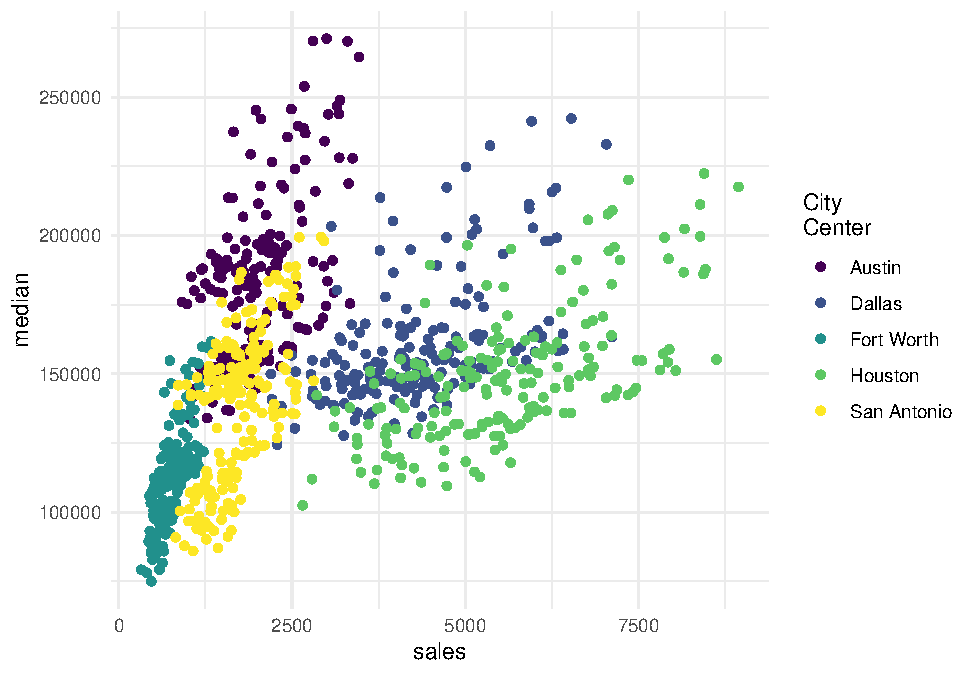
\includegraphics{/Users/alison/rprojs/rmd-render-factory/gallery/outputs/docs/latex_document_files/figure-latex/unnamed-chunk-2-1.pdf}

\hypertarget{austin-prices-on-the-rise}{%
\section{Austin prices on the rise}\label{austin-prices-on-the-rise}}

\begin{Shaded}
\begin{Highlighting}[]
\KeywordTok{ggplot}\NormalTok{(}\DataTypeTok{data =} \KeywordTok{filter}\NormalTok{(txsamp, city }\OperatorTok{==}\StringTok{ "Austin"}\NormalTok{), }\KeywordTok{aes}\NormalTok{(}\DataTypeTok{x =}\NormalTok{ sales, }\DataTypeTok{y =}\NormalTok{ median)) }\OperatorTok{+}
\StringTok{   }\KeywordTok{geom_point}\NormalTok{(}\KeywordTok{aes}\NormalTok{(}\DataTypeTok{colour =}\NormalTok{ year)) }\OperatorTok{+}\StringTok{ }
\StringTok{   }\KeywordTok{scale_colour_viridis_c}\NormalTok{(}\StringTok{"Austin by year"}\NormalTok{, }\DataTypeTok{option =}\NormalTok{ params}\OperatorTok{$}\NormalTok{viridis_palette, }\DataTypeTok{direction =} \DecValTok{-1}\NormalTok{) }
\end{Highlighting}
\end{Shaded}

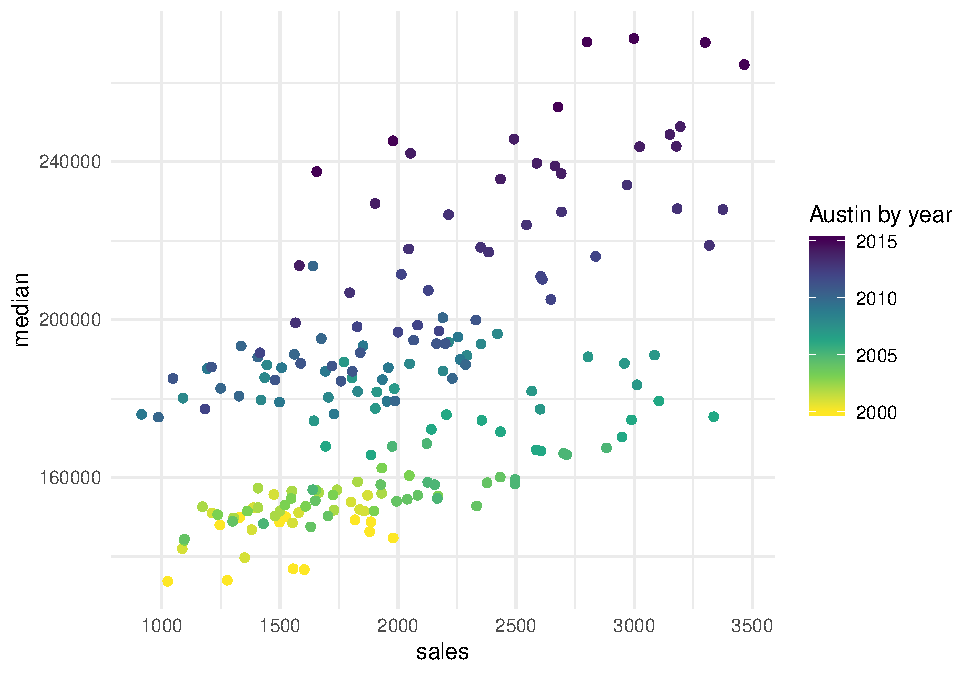
\includegraphics{/Users/alison/rprojs/rmd-render-factory/gallery/outputs/docs/latex_document_files/figure-latex/unnamed-chunk-3-1.pdf}

\hypertarget{fort-worth-has-more-affordable-housing}{%
\section{Fort Worth has more affordable
housing}\label{fort-worth-has-more-affordable-housing}}

\begin{Shaded}
\begin{Highlighting}[]
\KeywordTok{library}\NormalTok{(scales) }\CommentTok{# to make y-axis in non-scientific notation}
\KeywordTok{ggplot}\NormalTok{(txsamp, }\KeywordTok{aes}\NormalTok{(}\DataTypeTok{x =}\NormalTok{ median, }\DataTypeTok{fill =}\NormalTok{ city)) }\OperatorTok{+}
\StringTok{  }\KeywordTok{geom_histogram}\NormalTok{(}\KeywordTok{aes}\NormalTok{(}\DataTypeTok{weight =}\NormalTok{ sales), }\DataTypeTok{position =} \StringTok{"dodge"}\NormalTok{, }\DataTypeTok{binwidth =} \DecValTok{15000}\NormalTok{) }\OperatorTok{+}
\StringTok{  }\KeywordTok{scale_fill_viridis_d}\NormalTok{(}\DataTypeTok{option =}\NormalTok{ params}\OperatorTok{$}\NormalTok{viridis_palette)}\OperatorTok{+}
\StringTok{  }\KeywordTok{scale_y_continuous}\NormalTok{(}\DataTypeTok{labels =}\NormalTok{ comma)}
\end{Highlighting}
\end{Shaded}

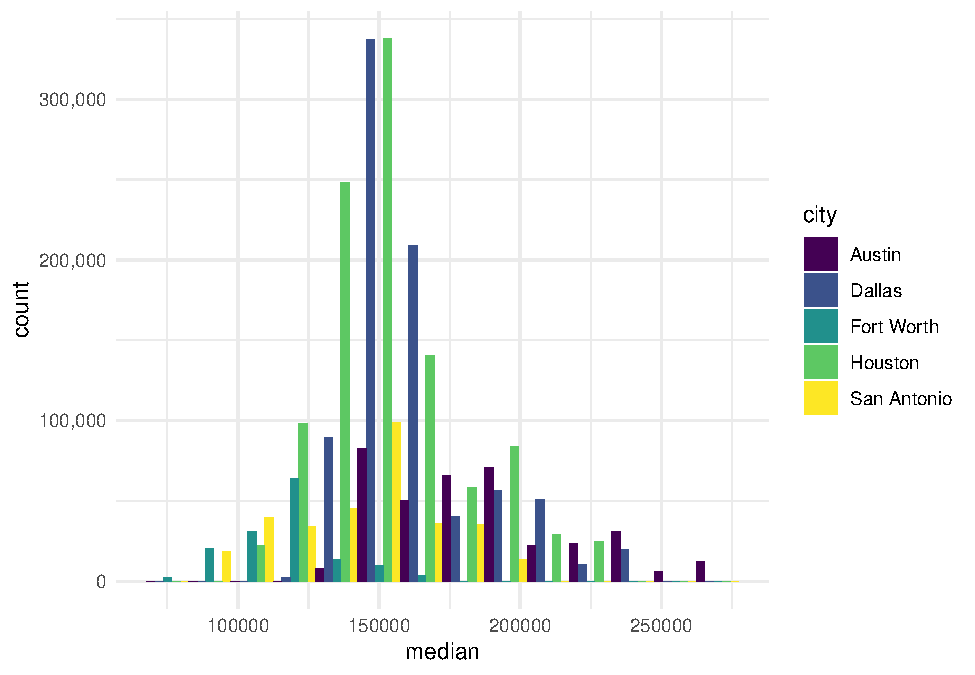
\includegraphics{/Users/alison/rprojs/rmd-render-factory/gallery/outputs/docs/latex_document_files/figure-latex/unnamed-chunk-4-1.pdf}

\hypertarget{the-current-pace-of-sales-is-fast}{%
\section{The current pace of sales is
fast}\label{the-current-pace-of-sales-is-fast}}

``Months inventory'': amount of time it would take to sell all current
listings at current pace of sales.

\begin{Shaded}
\begin{Highlighting}[]
\KeywordTok{ggplot}\NormalTok{(}\DataTypeTok{data =}\NormalTok{ txsamp, }\KeywordTok{aes}\NormalTok{(}\DataTypeTok{x =}\NormalTok{ year, }\DataTypeTok{y =}\NormalTok{ inventory, }\DataTypeTok{colour =}\NormalTok{ city)) }\OperatorTok{+}
\StringTok{  }\KeywordTok{geom_point}\NormalTok{() }\OperatorTok{+}\StringTok{ }
\StringTok{  }\KeywordTok{geom_smooth}\NormalTok{(}\DataTypeTok{se =} \OtherTok{FALSE}\NormalTok{) }\OperatorTok{+}
\StringTok{  }\KeywordTok{scale_colour_viridis_d}\NormalTok{(}\StringTok{"City}\CharTok{\textbackslash{}n}\StringTok{Center"}\NormalTok{, }\DataTypeTok{option =}\NormalTok{ params}\OperatorTok{$}\NormalTok{viridis_palette) }
\end{Highlighting}
\end{Shaded}

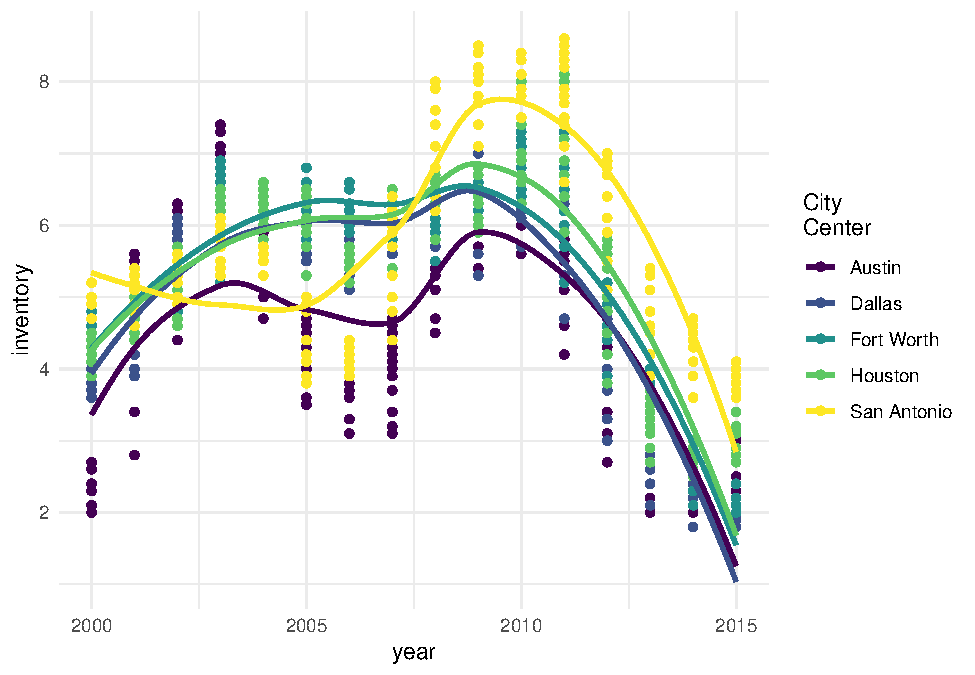
\includegraphics{/Users/alison/rprojs/rmd-render-factory/gallery/outputs/docs/latex_document_files/figure-latex/unnamed-chunk-5-1.pdf}

\hypertarget{thanks-to}{%
\section{Thanks to\ldots{}}\label{thanks-to}}

\begin{itemize}
\tightlist
\item
  Jennifer Thompson:
  \url{https://github.com/jenniferthompson/ParamRmdExample}
\item
  Garrett Grolemund: \url{https://rmarkdown.rstudio.com/lesson-6.html}
\end{itemize}


\end{document}
